\chapter{Introduction}\label{cha:intro}

\section{Motivation}

Synthetic data generation is a subject with increasingly high relevance.
The data can be used for training and validation of self-learning systems,
something which is becoming increasingly more popular and useful within vision
based problems. Solving methods for high speed generation of these datasets
can greatly increase the productivity and development of these
types of algorithms.

\section{Purpose}

For the purpose of generating synthethic data this thesis will investigate the use of physics
simulation for part distribution. The situation investigated in this thesis
is when several, identical models is  'poured' into a bin and simulated for their
final resting distribution. In figure~\ref{fig:plb}, the situation
the thesis aims to simulate is visualized. Only the distribution of the parts
will be simulated, i.e. the robotic arm and gripper used for picking the parts will not be simulated. For these simulations
performance is of high interest as generation of large amounts of data generation
is one of the key aspects. Due to the interest for performance a GPU method will
be investigated and compared to a more traditional CPU based solution.

\begin{figure}[ht]
  \centering
  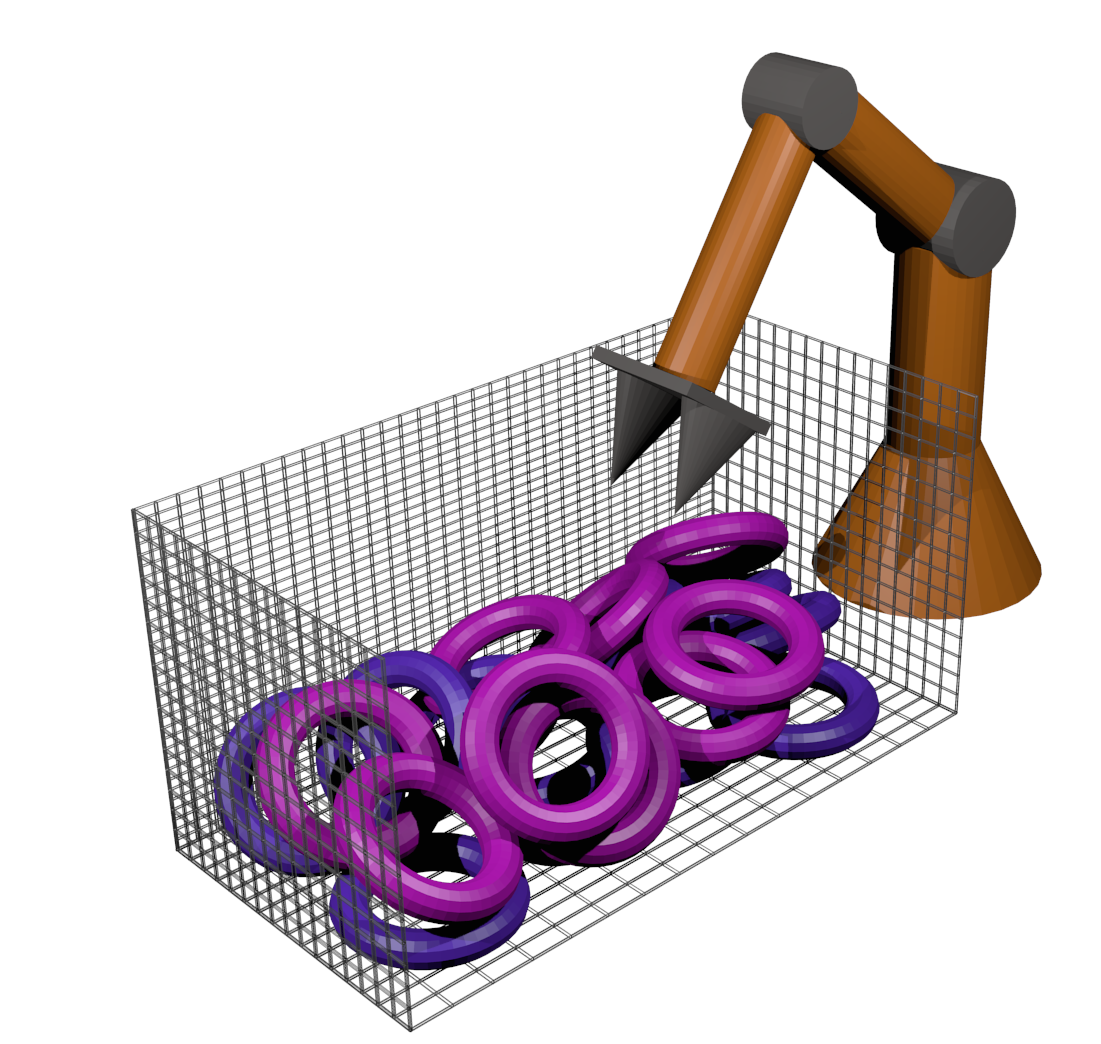
\includegraphics[width = 0.8\textwidth]{binBlender.png}
  \caption{The situation which the thesis aims to simulate.}
  \label{fig:plb}
\end{figure}

\section{Problem Statement}
How can a GPU rigid body solver be realised and used for synthetic data generation
 and how does it compare against Bullet?

\section{Limitations}
Since the system is somewhat chaotic in nature, deviations from a high accuracy
simulation in exchange for performance is accepted. The simulation should be reasonable
and the final distribution must be valid. For instance a detailed
model for the friction might not grant a better final distribution than a simple one.
Additional limitations are hardware. The methods will be evaluated on the hardware
provided by SICK IVP. Graphics card: GeForce GTX 960 with 4 GB GDDR5 VRAM.
CPU: Intel Xeon W3530 at 2.8 GHz.
Memory: 6 GB RAM.

Initially the Rigid-body GPU pipeline of Bullet 3.x was to be investigated, however
it has become apparent that the implementation was more or less abandoned in 2013
when Erwin Coumans started working for Google instead of AMD. While operational,
no API for it exists. Due to it's state it is excluded from the thesis.
A self-implemented GPU rigid body solver will be implemented and compared to Bullet.

\section{Methodology}
Validation for physics simulations is a very difficult topic. Since the aim for
the thesis is to produce realistic enough distributions we do not need to focus
on absolutely realistic results but can instead evaluate the results in terms of
a few key properties. Of interest are: performance, since the more images
that can be generated the better the chances of finding rare problems; correctness,
as the simulations need to be relatively correct to give rise to the problems that
 happen in real life scenarios; concave collision, since the objects might
 be concave and contain holes or other cavities.

The methods will be evaluated in a comparative fashion against one another.

Two CPU methods, the rectangle bounding-box and HACD will be implemented using
BulletPhysics 2.83, an open-source, permissively licensed, optimized game physics
library. The third method will be a GPU method implemented from scratch using a
voxelized particle method with impulses.
